\documentclass[12pt]{article}
\usepackage[T1]{fontenc}
\usepackage{sbc2003}
\usepackage{graphicx,url}
\usepackage[brazil]{babel}   
\usepackage[latin1]{inputenc}  

     
\sloppy

\title{}

\author{Cristiano Figueiró\inst{1} \and 
        Pedro Kroger\inst{1}}

\address{Genos---Grupo de Pesquisa em Computação Musical \\
         Escola de Música da Universidade Federal da Bahia \\
         Parque Universitário Edgard Santos, Canela \\
         40110-150 Salvador Bahia
         \email{figocris@gmail.com, pedro.kroger@gmail.com}
}

\begin{document} 
\graphicspath{{figs/}}
\maketitle

\begin{abstract}
\end{abstract}
     
\begin{resumo} 
  A música eletroacústica interativa em tempo-real, prevê uma série de
  desafios ao compositor ao exigir o cuidado na interação tímbrica, no
  controle dos eventos e forma e no fluxo de dados no mesmo projeto. O
  presente trabalho procura apresentar alguns aspectos particulares da
  criação de música interativa em tempo-real usando o software
  Pure-data (Pd). Serão abordados temas como as características de
  controle temporal e manipulação da forma como também técnicas
  clássicas de síntese sonora e manipulação de samples no Pd.
\end{resumo}


\section{Introdução}
\label{sec:introducao}


O presente artigo visa descrever a fase introdutória de meu projeto de
doutorado o qual trata da questão da interação em tempo-real entre
músicos e computadores através de um sistema computacional escrito no
software Pure-data. A música eletroacústica interativa (em
tempo-real), prevê uma série de desafios ao compositorao exigir o
cuidado nainteração tímbrica, no controle dos eventos e da forma e no
fluxo de dados no mesmo projeto. O presente trabalho procura
apresentar alguns aspectos particulares da criação de música
interativa em tempo-real usando o software Pure-data (Pd).

O Pure-data  é um ambiente de programação sonora e visual gráfico 
orientado ao objeto.O código é escrito em patches visuais, onde os objetos 
e seus controles são conectados via caixas com  entradas e saídas através de cabos.
O Pd pertence a família de programas oriundos do Max, que usam a metáfora
do fluxograma tradicional de síntese sonora como gramática da criação de patches.
O Pd  é escrito em C++ e aceita expressões de C++ como argumentos de controle.
É um software livre e multi-plataforma, além de contar com uma 
extensa comunidade de desenvolvedores. 

Esse projeto tem como objetivo fornecer informações no desenvolvimento
de uma composição escrita toda em Pd. onde todos os eventos sonoros
sejam determinados pela programação do próprio patch e não dependam de
interação com nenhuma fonte externa como teclado e mouse, entrada
de áudio em tempo-real e controle Midi externo. No processo de
aquisição de técnicas de programação musical em Pd, julgo importante
esse tipo de projeto pois apesar de todos parâmetros de eventos
estarem descritos estaticamente no patch, a música sempre ocorre em
tempo-real, ao contrário do Csound[Bou00] onde você edita o score e a
orchestra e depois compila o programa e confere o arquivo de áudio
resultante.
  
O paradigma composicional no Csound pode ser visto como semelhante ao 
trabalho tradicional do compositor que descreve eventos através de dois arquivos:
uma orchestra e um score, onde no primeiro são descritas as qualidades fixas do 
timbre e no segundo os eventos e os parâmetros dinâmicos do timbre. A arquitetura
de programas como Max e Pd, a primeira vista pode ser vista como simples e 
convidativa pelo fato de possibilitar uma programação intuitiva e parecer com 
um fluxograma. Mas logo se dão as primeiras dificuldades pelo fato de o paradigma 
da linguagem ser muito calcado na performance em tempo-real causando a
dificuldade de organização dos dados composicionais, como notas, acordes, eventos e
mudanças de parâmetros de síntese.

Os músicos tem sua formação baseada na notação musical tradicional que
estabelece uma cadeia de binômios de parâmetros de estruturação sonora\cite
{zampronha00:notacao} como altura
versus ataque, duração versus articulação ou métrica versus expressão. 
O sistema da notação tradicional tem uma
estrutura que possui uma sequencialidade temporal dos eventos
implícita. A migração dos músicos para ambientes de composição e
design sonoro como Csound \cite{boulanger00:csound} tende a ser mais natural pela
adaptação de um tipo de estrutura temporal (partitura) para outro
(Score), e também pela oposição binária entre "orchestra" e "score". No
Csound, a base de dados é chamada "Score". Scores em Csound consistem
na maioria das vezes em "notas", que são comandos para um sintetizador
(orchestra). O score é essencialmente uma sequência temporal. Uma possível
sequência temporal em Csound pode ser vista:

\begin{verbatim}
;orchestra
instr 1
  k1  linen 10000, .2, p3, .5
  a1  oscil k1, p4, 1
      out a1
endin

;score
f1 0 2096 10 1 .2 .3
i1 0 1 440
i1 1 1 660


\end{verbatim}

Programadores também são acostumados com linguagens de programação que
tem sua gramática baseada na sequencialidade das ações. A vantagem de
usar uma ferramenta de síntese embutida em uma linguagem de
programação é que se pode ter uma flexibilidade muito maior na criação
relações entre os elementos devido a possiblidade de criar novas
abstrações. Abaixo temos um exemplo de código em Comonn lisp music.



\begin{verbatim}
(definstrument simp (start dur frequency amp &optional
                    (amp-env '(0 0 .5 1.0 1.0 0)))
  (multiple-value-bind (beg end) (times->samples start dur)
    (let ((osc (make-oscil :frequency frequency))
          (amp-env (make-env :envelope amp-env :scaler amp
                             :dur dur)))
      (run 
       (loop for i from beg below end do
            (outa i (* (env amp-env) (oscil osc))))))))
\end{verbatim}

\begin{verbatim}
(with-sound ()
  (simp 0 1 440 1)
  (simp 1 1 660 1))
\end{verbatim}

\begin{verbatim}
(with-sound ()
  (loop for freq from 100 to 1000 by 100
     for dur from 0 to 10 do
       (simp dur 1 freq 1))
\end{verbatim}

Se formos tentar implementar esse código em Pd. Podemos encontrar algo assim: 

\begin{figure}[hp]
  \centering
  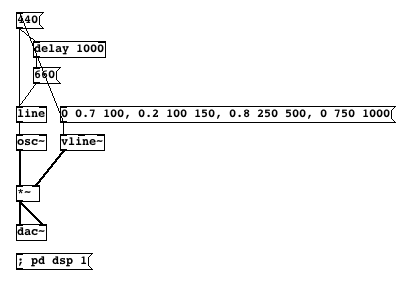
\includegraphics[scale=.5]{exemplopd1}
  \caption{2 notas num oscilador simples}
  \label{fig:exemplopd1}
\end{figure}

O fato do Pd ser uma linguagem gráfica possibilita uma facilidade de
descrição do processo de síntese sonora pelo fato de que o próprio
código é semelhante ao fluxograma tradicional de representação da
síntese (inserir figura de fluxograma). A estrutura de um fluxograma
possui uma sequencialidade implícita (da saída final até os parâmetros
de cada gerador), mas não explicita como vão ser manipulados os
parâmetros nem qual será a duração da música.

Os ambientes Max/Msp e Pd são construídos sob o paradigma do 
"envio da mensagem" que não necessariamente possibilita que a 
linguagem seja adequada para o estoque e a recuperação de dados. 
O usuário é praticamente forçado a colocar os dados dentro de conteiners - 
bases de dados, essencialmente - e a usar um leque de objetos como 
acessórios para estocar e recuperar dados dentro do controle de passagem 
de mensagens em tempo-real.

A abordagem do Max/ Msp quanto aos dados é ao mesmo tempo simples e
evasiva: objetos especiais de estocagem de dados como table, qlist,
etc...são disponibilizados; os dados são essencialmente
colocados dentro de objetos conteiners, e para cada tipo de
objeto-conteiner uma abordagem  particular é colocada para
sua estocagem, edição, interface e comunicação com o resto do patch.

Recuperação de dados (a grande maioria das transações de bases de
dados) é a pior qualidade do Max, porque mensagens não tem valores de
retorno (por exemplo, uma caixa de número manipulada com o mouse
não retorna os dados da manipulação, que devem ser recuperados com outros
objetos); os dados recuperados devem ser mandados como uma mensagem 
separada de retorno. Isso leva muitos programadores de Max a achar soluções
diferentes que facilite a interação do patch com o nível composicional.

A idéia original por trás da criação do Pd foi remover a barreira
entre a computação dirigida por eventos em tempo-real (como no estilo
do Max de passagem de mensagens) e dos dados (como em pontos num
gráfico ou notas numa partitura). Em Pd os dois (caixas de objetos e
estruturas de dados) podem facilmente coexistir em uma mesma janela.
Essa "promiscuidade", no entanto, não acaba deixando os objetos
funcionais e os dados intimamente conectados. De fato, no design
presente, o acesso aos dados tem que ser feito através de uma
sequência de objetos como acessórios . 

Em relação a essa divisão do aspecto "performático" e "composicional" do Pd,
Miller puckette explica \cite{puckette04:divide} : " In its most succinct form, 
the problem is that, while we have good
paradigms for describing processes (such as in the Max or Pd programs
as they stand today), and while much work has been done on
representations of musical data (ranging from searchable databases of
sound to Patchwork and OpenMusic, and including Pd's unfinished data
editor), we lack a fluid mechanism for the two worlds to
interoperate."

Dentro de uma proposta de trabalho de composição de música interativa,
o objetivo musical deve ser o mais claro possível de maneira que o
código emerja naturalmente dos problemas musicais ao invés de
atrapalhar mais ainda os problemas composicionais. Abordando o assunto
a partir de uma visão didático-metodológica um primeiro projeto
composicional em Pd, deve compreender a clara distinção entre os
aspectos performáticos e composicionais do ambiente. Um primeiro
projeto composicional deve dar conta de fornecer elementos para o
estabelecimento de uma metodologia apropriada de controle dos eventos
temporais. A proposta aqui é a de abordar o uso prático e algumas
possíveis implementações em Pd que apontem para a criação de
composições interativas mistas de maior porte. O objetivo é dispôr de
elementos que possam apontar para uma possível poética composicional.
Serão abordados temas como técnicas clássicas de síntese sonora e
manipulação de samples e também aspectos como controle temporal e
macro-estruturas no Pd.

\section{Técnicas de síntese e manipulação}
\label{sec:tecnicas-de-sintese}


 [texto introdutório]

\subsection{Síntese Aditiva}

A síntese aditiva pode ser entendida como o reverso da análise de Fourier. 
A figura \ref{fig:aditivo} mostra um exemplo típico de síntese aditiva em Pd onde os osciladores 
são somados em pares e tem a amplitude final controlada pelo objeto line~. Nesse caso 
cada oscilador poderia ter seus parâmetros de frequência (no caso fixos como argumentos 
numéricos escritos dentro das caixas de oscil~) e amplitude (objetos line~, ou outro 
gerador de envelopes) independentes uns dos outros..





\begin{figure}[hp]
  \centering
  \includegraphics[scale=.5]{aditivo}
  \caption{Síntese aditiva}
  \label{fig:aditivo}
\end{figure}

\subsection{Frequência  e Amplitude modulada}

Frequência e amplitude modulada são algumas das formas mais ricas de possibilidades tímbricas, onde a 
frequência, ou a amplitude respectivamente de um sinal de áudio é modulada por outro sinal de áudio. 
Na figura\ref{fig:modulada}, abaixo os parâmetros da síntese são controlados por caixas de números e 
slides. No caso, uma possível interação em tempo-real com um instrumentista poderia prever o endereçamento 
dos valores de frequência e amplitude do sinal de áudio de entrada para agendar respostas sonoras variando os 
valores dos parâmetros baseados nos dados do áudio de entrada.

\begin{figure}[hp]
  \centering
  \includegraphics[scale=.5]{exfm1}
    \includegraphics[scale=.5]{exam1}
  \caption{frequência modulada}
  \label{fig:modulada}
\end{figure}



\subsection{Manipulação de samples}
\label{sec:manip-de-sampl}
Sampling é uma técnica simples de ser realizada no Pd. O endereçamento de samples externos é feito apenas 
salvando os samples no mesmo diretório em que o patch que os usa está salvo. Na figura 
\ref{figurasamples} o objeto “soundfiler” faz a leitura de samples a partir da mensagem “read”, o sample 
no caso é endereçado para um “array”, onde é especificado o tamanho do arquivo que vai ser lido. Os samples 
são manipulados por três módulos. O primeiro realiza um “scratch” (“surfa” pelo sample) através de um 
“line~” que tem seu parâmetro controlado em tempo real por uma caixa de número (no caso é uma das 
variáveis dessa abstração e está conectada a um “line”, controlado por diferentes valores de “metro”).  
O segundo módulo realiza um loop com “tabplay~” que é um objeto que manda um “bang” quando acaba 
de tocar o sample especificado. O terceiro módulo é um loop com “tabread4~” controlado por “phasor” que 
manda um sinal contínuo de áudio podendo transpôr a altura do sample.

\begin{figure}[hp]
  \centering
  \includegraphics[scale=.5]{sample2}
  \caption{}
    \label{fig:}
\end{figure}

\section{Fluxo de dados}
\label{sec:fluxo-de-dados}

Uma das partes mais importantes de um projeto composicional com Pd é o controle do fluxo de dados,
 pelo fato de que o programa não tem uma sintaxe uniforme de descrição de eventos, e cada objeto específico 
 vai ter uma gramática própria de controle de dados. Na figura \ref{fig:extempo1} vemos um gerador 
 “osc~” sendo modulado por um gerador de envelopes de sinal de áudio “vline~”. Esse gerador de envelopes 
 agenda segmentos lineares e possui uma sintaxe que aceita trios de números, sendo respectivamente:
  amplitude (objetivo de chegada do segmento) ,tempo inicial (tempo de começo do segmento) e tempo 
  de duração do segmento. A recuperação dos dados da performance de “vline~” é feita pelo objeto 
  “snapshot~” que transforma dados de sinal de áudio em números. O objeto “snapshot~” por sua vez é 
  acionado pelo objeto “metro” que é um controlador temporal que manda “bangs” (mensagem: “faça”) 
  regulares no andamento especificado pelo seu argumento descrito em milisegundos. O seja, “vline~” 
  vai envelopar a amplitude de “osc~” enquanto “snapshot” vai fazer leituras do fluxo de áudio numa 
  frequência de 10  vezes por segundo.

\begin{figure}[hp]
  \centering
  \includegraphics[scale=.5]{extempo1}
  \caption{}
    \label{fig:extempo1}
\end{figure}


\subsection{Abstrações e subpatchs}
\label{sec:abstr-e-subp}
Na figura \ref{fig:2a} está exposta uma abstração que tem a função de mandar um 
“bang” no tempo pré-estabelecido (argumento de delay). Essa abstração está sendo usada
 na peça para “desligar” os módulos geradores no tempo especificado. Abstrações são patchs
 que assumem funções de objetos externos e podem ser usados por vários patchs diferentes 
 ao mesmo tempo. Além disso possibilitam um certo controle gráfico, definido pelo 
 programador. No caso, vemos que no patch temos um “bang” e uma “caixa de número” 
 contidos num retângulo, consequentemente quando essa abstração for chamada num patch 
 vai assumir a forma da figura \ref{fig:2b}.
\begin{figure}[hp]
  \centering
  \includegraphics[scale=.5]{ex2a}
  \caption{}
    \label{fig:2a}
\end{figure}

\begin{figure}[hp]
  \centering
  \includegraphics[scale=.5]{ex2b}
  \caption{}
    \label{fig:2b}
\end{figure}

\subsection{Objetos de controle temporal}
\label{sec:objetos-de-controle}

\begin{figure}[hp]
  \centering
  \includegraphics[scale=.5]{forma}
  \caption{}
    \label{fig:forma}
\end{figure}

\section{Compondo com o PD}
\label{sec:compondo-com-o}



Uma vez tendo prontos os geradores sonoros e os controladores dos
dados desses geradores - em formatos de abstrações e/ou sub-patchs,
podemos pensar em controlar a macro-forma da composição. Na figura
\ref {fig:forma} está exposto o controle da macro-forma da peça. Essa maneira
visual de controlar a forma é mais familiar aos músicos pelo fato de
termos uma linha do tempo mostrando a ordem de acontecimento dos
eventos. O que permite uma maior controle de justaposição e
superposição dos macro-eventos. A abstração "contador", cria um novo
número no andamento específico e o objeto "select" cria pontos
temporais de ataque que são endereçados a diferentes geradores
sonoros.

\begin{figure}[hp]
  \centering
  \includegraphics[scale=.5]{gerador}
  \caption{}
    \label{fig:gerador}
\end{figure}

A figura \ref{fig:gerador} mostra o patch encapsulado “pd gerador1 gerador2”, que apareceu
na figura \ref{fig:forma} e tem seu gerador sonoro baseado em síntese aditiva. O controle é 
feito por uma combinação dos objetos line e metro, onde o line controla o parâmetro 
de tempo de  metro, causando linhas de acelerando ou desacelerando. O momento de 
“desligamento” de cada gerador é agendado pela abstração “delayabs”.

\section{Conclusão}
\label{sec:conclusao}


A composição em Pd tem como característica a facilidade do controle de síntese, porém exige
um tratamento especial na metodologia empregada no controle de eventos temporais. 
Segundo\cite{puckette04:divide}:
"The Pd patch looks more complex than the C code. One possible reason for
the complexity is the dificulty of sequencing actions in Pd patches, which lack
the natural sequentiality of a text programming language like C. “
O fato de cada objeto  de controle temporal apresentar uma sintaxe diferente
pode ser antes um convite a criatividade composicional do que um problema estrutural
da música resultante.
%%%%%%%%%%%%%%%%%%%%%%

\nocite{*}

\bibliographystyle{apalike}
\bibliography{bibliografia}

\end{document}
